%%%%%%%%%%%%%%%%%%%%%%%%%%%%%%%%%%%%%%%%%%%%%%%%%%%%%%%%%%%%%%%%%%%%
% Basic Informations
%%%%%%%%%%%%%%%%%%%%%%%%%%%%%%%%%%%%%%%%%%%%%%%%%%%%%%%%%%%%%%%%%%%%

\chapter{Basics}\label{Basics}
% todo explain EA, Gene, Genome, Allel. 


\section{NEAT}\label{NEAT} % todo paper reference
\Gls{neat} (\cite{NEAT}) is an neuroevolution method that genetically encodes and evolves weights and topologies of neural networks. \gls{neat} stands out from other neuroevolution algorithms by meaningful crossovers in disparate ANN topologies, protection of topological innovations and a efficient search by a stepwise increasing search space. (TODO cite some). Furthermore \gls{neat} is well suited for reinforcement learning problems. 
\subsection{biological basics} 
% maybe definitions are better ask %MKK zitieren %% todo fachwerk aus bib
The whole inheritable information needed to create a new organism is called genome. A genome consists of genes which are responsible for the expression of specific features. Genes that express same features with  different characteristics are called alleles. Assuming the eye colour is expressed by one gene.  Variations of this gene which lead to different eye colours are alleles. (TODO find proven example with one gene)
\subsection{Evolutionary algorithm} % Todo abkürzung EA
Evolutionary algorithms (EAs) (see generally \cite{book:IntroductionEA}) are algorithms that mimic the natural evolution process. That is that only the fittest organisms of a generation will survive. An EA maintains a group of solutions called a population. A solution in a population is called an individual. Each individual has a numerical fitness value that determines how good this solution is. An individual is represented by a code also called genome. During the run of an EA a genome of an individual undergoes several variation operations. One typical operations are mutations, where parts of the genome are changed randomly. Cross Over as an other typical operation exchanges parts of the genome of two individuals. Usually an EA performs those operations to generations and only the fittest childs are s taken over into a new generation. The function giving the fitness of an individual is called objective function. EAs are mainly used to find good local maxima of objective functions that are either unknown or not analytical differentiable and not solvable with numerical methods like gradient descends.  (TODO nachlesen vergleichn script zell)
TODO typischer evolutionszykel erklären.


\subsection{operating principle} 
The genetic basic of \gls{neat} is a direct encoded genome, which contains connection and node genes. Each node gene evolves a neuron while each connection gene represents a weighted and directed connection between two neurons. A node gene contains it's identification number and it's type. Possible types are Input, Output and Hidden. A connection gene encodes its connection by referring to two node gene identification numbers. In addition a connection gene contains its weight, an expression flag and an innovation number. The expression flag indicates whether the expression gets realised or not. The innovation number is the fixed identification number of a connection gene. Alleles of a connection gene share the same node genes and innovation number but can have different weight and expression flag values. Every time a new neuron gene or connection gene is created a global counter number is increased by one and than used as the new innovation number. In the case that the same connection gets created in two different offsprings of a generation they get the same innovation number assigned. This only applies if it happens in the same generation. Thus one gene can only evolve in one particular generation. As a result the innovation number assures that connection genes with the same innovation number connect the same nodes but not all connection genes connecting the same nodes have the same connection number.(this represents the biological fact, that the same feature can be expressed by different genes.). An example for a NEAT genome is depicted in figure \ref{fig:neatgenome}.\\
Three types of mutation are realized. A \textit{weight mutation} mutates each weight mutates with the same probability. New connections are added by the add connection mutation. Thereby two unconnected cells are randomly chosen and connected by a new connection gene with a random weight. A new cell mutation splits an existing connection by placing a new node between the two former connected nodes. This is realized by disabling the old connection gene and the creation of two new connection genes and one new node gene. One connection gene connects the input node with the new node and gets its weight set to the value of the former connection. The other connection gene is connects the new node with the output node of the former connection and gets its weight set to one. This expression of weights leads to an minimized initial effect of a mutation. Two exemplar mutations are displayed in figure \ref{fig:neatmutations}.\\
In? a cross over at first a synapsis is done. This means that all connection genes of two individuals are lined up. Genes that have the same innovation number are called matching genes. Genes of one individual which innovation numbers are inside the range of the other individual matching genes' innovation numbers are called disjoint genes. Innovation numbers outside the range of the other individual matching genes' innovation numbers are called excess genes. The child's genome is created by selecting one gene randomly out of each tuple of matching genes, disjoint and access genes are taken from the more fit parent. With a preset probability a disabled gene can be enabled again when it is disabled in both parents. By crossing over only connections and no whole substructures of the network (like other approaches do  TODO find one vorlesung Zell trees), it is ensured that a new proper artificial neural network is created. 
An exemplar cross over of two individuals with the same fitness is shown in figure \ref{fig:neatcrossover}. \\
Specitation: 
Based on empirical evidence insertion of new structures into a network leads at first to a decrease in fitness. Thus its unlikely that the individual can compete against others in this generation and will be distinct. A new structure needs some time to adapt its weights in a way that the new structure is beneficial. Thus specitation also known as niching is implemented in NEAT to protect new structure. Similar individuals are put in their own species. Members of a species are primarily competing against each others. That means artificial neural networks with similar structures are primarily competing against each other. To determine to which species an individual belongs the following distance measurement between two aligned individuals is used:
\begin{equation*} 
\delta = \dfrac{c_1E}{N}+\dfrac{c_2D}{N}+c_3*\overline{W}.
\end{equation*}
Where $E$ is the number of excess genes and $D$ the number of disjoint genes. $\overline{W}$ is the average of weight differences of all matching genes. The normalization factor $N$ is the number of genes of the larger genome. $c_1$,$c_2$,$c_3$ represent scaling factors. 
In detail a ordered list of species is given. For the next generation one representative individual is randomly chosen out of each species. Each member $m$ of the next generation is compared consecutively to these representatives. If the distance measurement $\delta$ is smaller than a fixed threshold $\delta_t$, $m$ is put into the species of the representative. If $m$ is not compatible to any representative a new species with $m$ as its representative is created. This way assures disjunct species.
To prevent that one species takes over the entire population explicit fitness sharing (TODO link Golsberg and Richardson 1987) is used. For each individual $i$ its adjusted fitness $f_{i}^{'}$ is calculated the following way:
\begin{align*} 
f_{i}^{'}&=\dfrac{f_i}{\displaystyle\sum_{j=1}^{n} sh(\delta(i,j)) }\\
sh(i,j) &= \begin{cases}
1 & \quad \text{if } \delta(i,j) < \delta_t \\
0 & \quad \text{if } \delta(i,j) \geq \delta_t
\end{cases}
\end{align*}
Where $f_i$ is the fitness of $i$, $\delta(i,j)$ the distance between individual $i$ and $j$. And $sh$ a sharing function that determines whether $i$ and $j$ are in the same species.
As a result under the assumption that the fitness function has no plateaus at local maxima the shared fitness of species members is decreased if the species gets larger. Every species produces a number of offsprings $NO$ proportional to the sum of adjusted fitnesses $f_{i}^{'}$ of its members. The total amount of offsprings is limited by the maximum population size $P$ and the number of individuals that are taken over directly from the last generation $L$.
\begin{equation*} 
NO(s) = (P-L)\cdot\dfrac{\displaystyle\sum_{\forall i \in s} f_{i}^{'}}{\displaystyle\sum_{\forall i } f_{i}^{'}}
\end{equation*}
  %TODO bei zell im script nachlesen -> verbessern.
\\ NEAT starts with a minimal structure. That is, each input neuron and one optional bias neuron is connected with each output neuron. There are no hidden neurons. Starting with a minimal structure leads to an efficient search. Since add node mutations and add connection mutations are rare compared to weight mutations the search space is increased slowly. The search space consists of one dimension for each weight and one dimension representing the number of neurons. That means starting with a minimal network networks with increasing complexity are considered as solution for the problem.


 
  
  
\begin{figure}[tb]
	\centering
	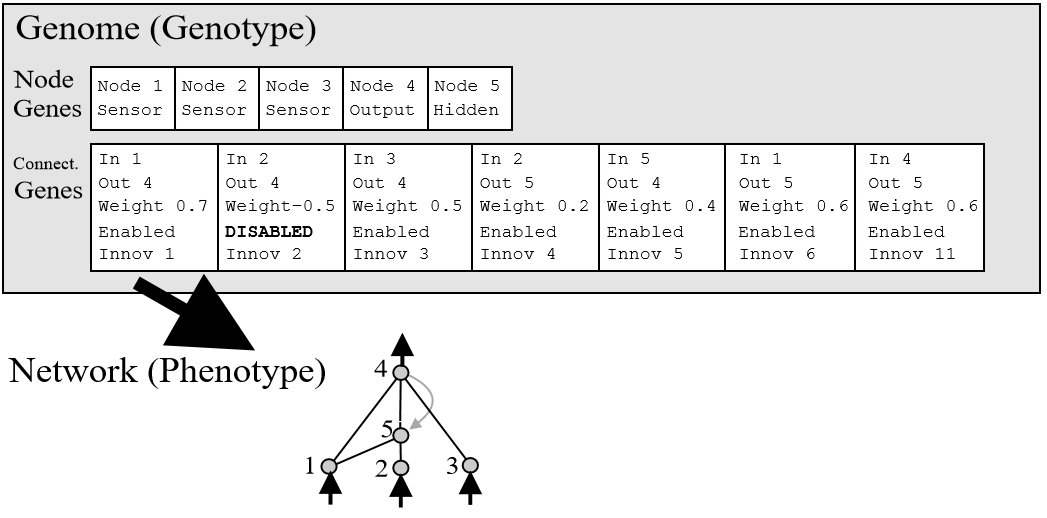
\includegraphics[width=0.7\linewidth]{figures/NEAT/NEATGenome}
	\caption[NEAT genome]{NEAT genomes consist of two type of genes: node genes displayed in the first row and connection genes displayed in the second row. Each node gene has an identification number (first element) and one of three types: sensor (input), output and hidden. A connection gene contains its input and output node, a weight, an expression flag and a innovation number. Underneath the genome the resulting network is displayed. The numbers are identical to the node IDs. Enabled connections are displayed black. Disabled connections are shown grey. \cite[p. 106]{NEAT} }
	\label{fig:neatgenome} % TODO wirklich so ausführlich wiederholen notwendig?
\end{figure}
  
  
  
\begin{figure}[tb]
	\centering
	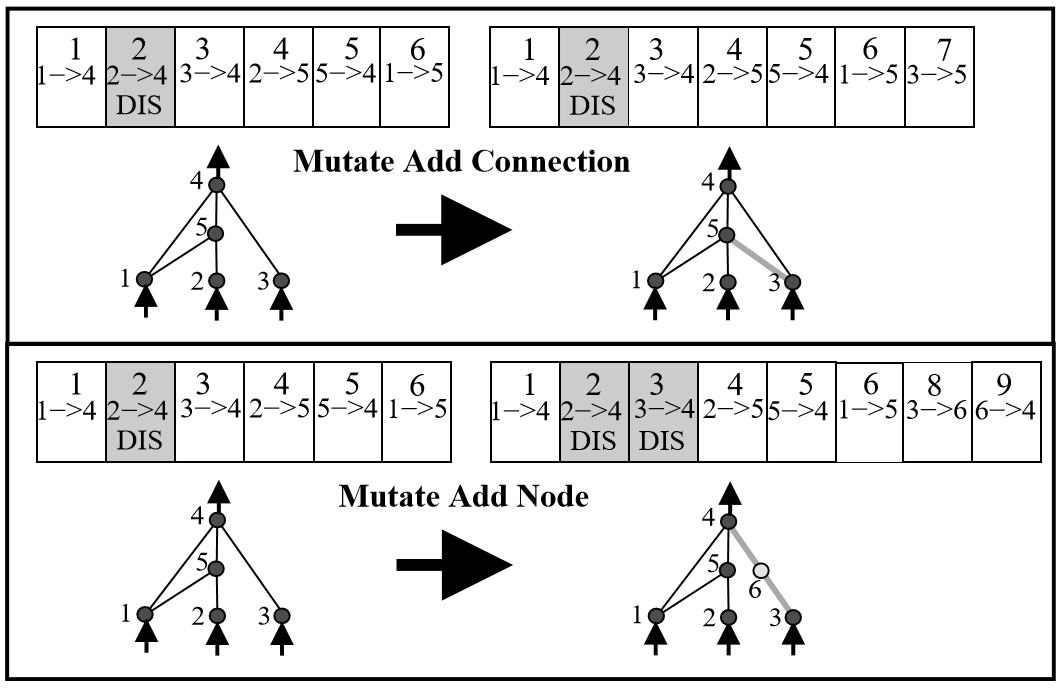
\includegraphics[width=0.7\linewidth]{figures/NEAT/NEATMutations}
	\caption[NEAT mutations]{At the top a add connection mutation is displayed. The unconnected nodes 3 and 5 are chosen randomly. Then a connection gene between  those nodes is created. The global innovation counter number is increased by one (from 6 to 7) and allied to the new connection gene.\\
	At the bottom a add node mutation is displayed. Connection 3 is randomly chosen and gets disabled. Next a new node gene with ID 6 is created. Then fist new connection gene connecting  node 3 and 6 with innovation number 8 and a second connecting node 6 and 4 with innovation number 9 is created. \\
Note that only connection genes are displayed. The top number in each gene is its innovation number followed by the node it connects and the expression flag.
Node genes are not depicted.
\cite[p. 107]{NEAT}}
	\label{fig:neatmutations}
\end{figure}
  
  
  
\begin{figure}[tb]
	\centering
	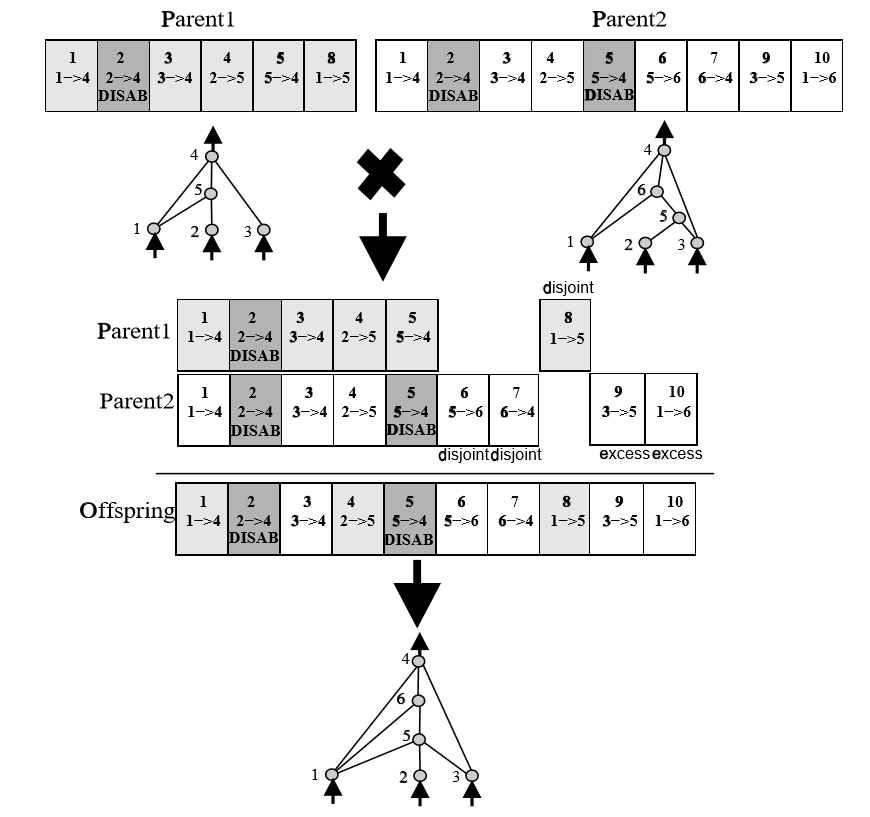
\includegraphics[width=0.7\linewidth]{figures/NEAT/NEATCrossOver}
	\caption[NEAT cross over]{Two individual's connection genes and their corresponding networks are displayed at the top. Underneath this two genomes got aligned. All connection genes with same innovation numbers are displayed opposite each other. Those are matching genomes. All connection genes of one individual that are in the range of the other individual's connection gene are marked as disjoint. Connection genes that are outside the range of the other individual's connection gene are marked are marked as excess. The offspring's connection gene consists of one randomly chosen connection gene out of each matching gene. In this example the fitness of both parent individuals is equal. Thus all excess and disjoint connection genes are chosen. If the fitnesses would differ the excess and disjoint connection of the more fit parent are taken over.\cite[p. 109]{NEAT}}
	\label{fig:neatcrossover}
\end{figure}
  
  
Neuroevolution is a machine learning technique that evolves weights and topology of artificial neural networks by means of evolutionary algorithms. 

TODO: explain 
Neuroevolution
evolutionary algorithm


"Neuro-evolution of augmenting topologies (NEAT) is a method for genetically encoding and evolving the architecture and the weights of neural networks "

\section{HyperNEAT}\label{HYPERNEAT}
\subsection{Basic HyperNEAT}
\subsubsection{Scaling}
\subsubsection{Modulation}
\subsection{ES HyperNEAT}\label{ES_HYPERNEAT}

\section{Motorcortex Model}\label{MotorCortex_Model}